% !TEX root = ../main.tex

\section{Discussion}
In this section we discuss the remaining results from our grounded theory work.

% Jeremy: leverage of multiple use cases on teh same blockchain

\subsection{Normative properties}
\label{sec:normative}

\begin{figure}
	\centering
	\includegraphics[page=3,width=\columnwidth]{figures/grounded-theory-main}
	
	{\small Orange---normative properties, purple---capabilities, blue---technical properties, green---technical primitives. Arrows indicate that the destination depends on the source.}
	\caption{Normative Properties for Blockchain Technology}
	\label{fig:normative-properties}
\end{figure}

Within the literature we analyzed, there were a set of properties that were not technical properties directly provided by Blockchain technology, but rather expressed desired properties for systems built using Blockchain technology (\ie normative properties).
These properties are shown in Figure~\ref{fig:normative-properties}.

The majority of the normative properties focused around the notion of using Blockchain technology to allow for public participation.
While public participation is certainly possible with Blockchain technology, as there are many example of systems built using Blockchain technology that fail to achieve these properties.
For example, while Bitcoin initially had a low-cost to participate allowing easy-of-entry for miners and community ownership, that is no longer the case as any meaningful participation requires the purchase of a large amount of specialized hardware and the expenditure of a significant amount of electricity.

Similarly, the normative properties of low-bar for trust, disintermediation, no trusted third-parties, censorship resistance, and fast/cheap transaction all require extremely careful system design to achieve, and are not guaranteed by the use of Blockchain technology.
In practice, these properties are often difficult to guarantee for any system, and this is no different for Blockchain technology.
For example, Bitcoin ultimately requires trusted third parties (e.g., exchanges, retailers who accept Bitcoin) to allow the currency to be useful for real-world application.
Also, fast/cheap transactions usually only exist because Blockchain based systems are not yet regulated like non-Blockchain systems.

When reading documents from industry, normative and technical properties are often intermingled with each other.
The injection of ideology into a technical field causes confusion and suboptimal design choices, not to mention muddying discussion and preventing clarity.
Interestingly, in the concept graph generated by our methodology, the technical and normative properties were cleanly separated.
No capabilities have dependencies on normative properties, and removing them from the graph does not lessen the value of the graph as an exploration of technical concepts.
The fact that this separation occurred naturally provides evidence that grounded theory accomplished our research goals and was a good choice for addressing this corpus of data.

%In general, the normative properties dealt with idealogy-driven goals that could be accomplished using Blockchain technology.
%For example, several normative properties dealt with public participation, community ownership, censorship resistance, and transparency of Blockchain systems.
%Bitcoin demonstrates that Blockchain technology can be used to achieve these properties, but it is not the case that all Blockchain systems will accomplish these goals---for example, Ripple is a Blockchain system without public participation.

\subsection{Private Governance}
\label{sec:private-blockchain}
In our survey of the industrial literature, we encountered several proposals for Blockchain technology that used a centralized governance model where all miners are controlled by a single entity.
The most prominent example of a private governance system is IBM's HyperLedger Fabric.
Interestingly, the HyperLedger Fabric software project allows for consortium governance, but IBM's implementation has IBM run all of the miners.

Ultimately, we do not classify such systems as Blockchain technology.
First, these systems do not neither shared governance nor shared operation, which we identify as the key component of Blockchain technology.
Second, the entity operating the system still represents a single-point of failure.
While the miners within the operating organization might be run on a distributed infrastructure, there is still a high chance that a compromise in the operating organization would lead to a compromise in the Blockchain system.
Third, there is nothing that prevents the governing party from deleting or modifying data; even if such changes could be detected, the data itself is not replicated outside the organization and would be lost.
This is not to say that such systems lack value---such an evaluation is beyond the scope of this paper---but rather we believe that these types of systems are distinct from the more decentralized Blockchain technology.

\subsection{Lack of Privacy and Data Discoverability}
In the literature we found a common misconception that Blockchain technology inherently provided confidentiality for information stored within it.
In fact the opposite is true: all transactions are visible to all miners, and this is necessary for miners to validate transactions.
The global visibility was identified by some as a capability (i.e., data discoverability) that allowed a Blockchain to act as a data lake.
While there were some valid applications of Blockchain as a data lake, in most cases we found that proposed data lake applications did not need all of Blockchain technology's capabilities and that a simpler solution would have sufficed.
It may be possible to add confidentiality to Blockchain technology, but care must be taken to ensure that this confidentiality does not preclude miners' ability to validate and audit the system.
This remains an open research problem.

\subsection{Ideology, Hype, and Ulterior Motives}
Many proponents of Blockchain technology believe that it has the capability to massively disrupt how society operates, or at least to rapidly overtake legacy solutions in many significant industries. This belief is hyperbole, as though Blockchain technology has many valid uses, it has not, nor is it likely to achieve this Utopian vision. This ideology and hype causes problems: for example, frequent emotionally-charged schisms within Blockchain advocate and developer communities---especially those affiliated with Bitcoin. This turmoil prevents level-headed scientific discourse and wastes developer resources. It can also tangibly affect the stability of a Blockchain system by causing a fork in which two independent chains emerge to used and maintained by different groups, further dividing resources.

With that said, Blockchain's disruptive power has certainly been demonstrated in the financial sector, so it clearly has promise. Several factors have made this sector an attractive target for disruption, perhaps none more so than the opportunity for massive profit. This motive has had benefits for Blockchain, especially in accelerating the pace of technological development. However, it has also created perverse incentives to reinforce hype and ideology. Hype can attract investors and inflate valuations, and dogmatic ideology is a proven marketing and recruitment strategy for financial scammers. These problems inhibit the advancement of Blockchain technology.

\subsection{Reputation for illicit uses}
Due to the prominence of Bitcoin, many people are familiar with Blockchain first and foremost as the technology underlying the cryptocurrency and therefore the reputations of the two are intertwined. The fact that Bitcoin is designed to avoid banks and central authorities in general, combined with its well-known history of illicit uses, somewhat poisons the well for Blockchain as a whole. Along with the causes listed above (ideology, hype, and ulterior motives), this contributes to the difficulty of discussing and considering Blockchain technology with precision and objectivity. It may also have impeded or delayed its acceptance by organizations unwilling to associate themselves with the Bitcoin's poor reputation.